\section{Sintesi e caratterizzazione con 1H NMR di \ce{[Co(dinosar)]Cl3}}
\subsection{Sintesi \ce{[Co(en)3]Cl3}}
\subsubsection{Procedura sperimentale}
Abbiamo preparato una prima soluzione disciogliendo 6.02 g di \ce{CoCl2.6 H2O} in 17.5 mL circa d’acqua prelevata con un cilindro graduato. In contemporaneamente, abbiamo sciolto in un altro becher 5 mL (4.5 g) di etilendiammina in 12.5 mL di acqua. Quindi abbiamo acidificato la soluzione di etildiammina con 4.5 mL di acido cloridrico 6 M in un bagno di ghiaccio. Abbiamo unito le due soluzioni e abbiamo aspettato mezz’ora che avvenisse la complessazione. In seguito abbiamo aggiunto goccia a goccia 5.0 mL di acqua ossigenata al 30\% per ossidare il centro metallico. Al termine dell’effervescenza abbiamo svaporato a 30 mL e aggiunto lentamente 30 mL di HCl 12 M e 60 mL di etanolo. È precipitato un sale giallo ocra che abbiamo filtrato su Buchner, lavato con etanolo (3 × 10 mL). Abbiamo raccolto il prodotto in una provetta precedentemente pesata e l'abbiamo seccato sottovuoto.

\subsubsection{Commenti e osservazioni}
Durante l'acidificazione dell'etildiammina con HCl abbiamo notato la formazione di fumi bianchi. Questi si presume dovuti all'etildiammonio cloruro prodotto dalla reazione dell'acido cloridrico gassoso con etildiammina passata in fase gas per il riscaldamento della soluzione dovuto all'esotermicità della reazione di acidificazione. L'acqua ossigenata utilizzata era stata tenuta in frigo, i perossidi sono sostanze sensibili e tendono a decomporsi.


\subsubsection{Calcoli e analisi dei dati}
In partenza avevamo un numero di moli di reagenti pari a
$$
\begin{gathered}
n_{\mathrm{CoCl}_2}=\frac{6.00 \mathrm{~g}}{237.93 \mathrm{~g} / \mathrm{mol}}=0.0253 \mathrm{~mol} \\
n_{\mathrm{en}}=\frac{5 \mathrm{~mL} \cdot 0.899 \mathrm{~g} / \mathrm{mL}}{60.10 \mathrm{~g} / \mathrm{mol}}=0.07479 \mathrm{~mol}
\end{gathered}
$$
La stechiometria della reazione è 1 : 3 notiamo che il reagente limitante è l'etilendiammina\footnote{E' il reagente limitante per poco. }.
Calcoliamo la resa 
\[ Y_\% = \frac{n_\text{pro}}{n_{\mathrm{CoCl}_2}}\cdot 100 \]

Le moli finali sono il rapporto massa della provettà piena di prodotto tolta la tara e la massa molare del prodotto.

\[ n_\text{pro} = \frac{(m_{f\#1} - m_{t\#1})+(m_{f\#2} - m_{t\#2})}{M_\text{pro}} 
 = \frac{ 3.7564 \um{g} + 4.1124 \um{g} }{ 345.58 \um{g/mol}} =  \frac{7.8688 \mathrm{~g}}{345.58 \mathrm{~g} / \mathrm{mol}}=22.77 \um{mmol}\]

\[ Y_\% = \frac{n_\text{pro}}{n_{en}}\cdot 100  = \frac{3 \cdot 22.77 \cdot 10^{-3} \mathrm{~mol}}{74.79 \cdot 10^{-3} \mathrm{~mol}} \cdot 100 =91.3\%\]


\subsection{Sintesi \ce{[Co(dinosar)]Cl3}}
\subsubsection{Procedura sperimentale}
Abbiamo sciolto $2.45 \mathrm{~g}$ esatti del prodotto del passaggio precedente in $25 \mathrm{~mL}$ di acqua con $1.20 \mathrm{~g}$ di carbonato di sodio. Abbiamo quindi aggiunto $18 \mathrm{~mL}$ di formaldeide al $40 \%$ prelevata con un cilindro e $2.5 \mathrm{~mL}$ (circa $2.8 \mathrm{~g}$) di nitrometano. Dopo aver lasciato la soluzione a temperatura ambiente per qualche ora l'abbiamo riscaldata per un'altra ora al minimo della piastra elettrica. Abbiamo quindi filtrato su Buchner e recuperato il precipitato arancione che abbiamo ricristallizzato da una soluzione in $\mathrm{HCl} $ 3M. Infine, dopo aver aggiunto etanolo come non solvente abbiamo filtrato su Buchner, seccato all'aria, trasferito in una provetta di massa nota e seccato sottovuoto.
\subsubsection{Commenti e osservazioni}



\subsubsection{Calcoli e analisi dei dati}
In partenza avevamo un numero di moli di reagenti pari a
\[ n_{\ce{[Co(en)3]Cl3}}=\frac{2.45 \mathrm{~g}}{345.58 \mathrm{~g} / \mathrm{mol}}= 7.090 \mathrm{~mmol} \]

\[ n_{\mathrm{HCOH}}=\frac{18 \mathrm{~mL} \cdot 1.09 \mathrm{~g} / \mathrm{mL} \cdot 40 \%}{30.03 \mathrm{~g} / \mathrm{mol}}=0.26 \mathrm{~mol} \]
\[ n_{\mathrm{CH}_3 \mathrm{NO}_2}=\frac{2.5 \mathrm{~mL} \cdot 1.127 \mathrm{~g} / \mathrm{mL}}{61.04 \mathrm{~g} / \mathrm{mol}}=0.0462 \mathrm{~mol} \]

Considerando quindi la stechiometria $1: 6: 2$ notiamo che il complesso il reagente limitante. Abbiamo ottenuto $ 2.675 \mathrm{~g}$ di prodotto



Calcoliamo la resa 
\[ Y_\% = \frac{n_\text{pro}}{n_{\ce{[Co(en)3]Cl3}}}\cdot 100 \]

Le moli finali sono il rapporto massa della provettà piena di prodotto tolta la tara e la massa molare del prodotto.

\[ n_\text{pro} = \frac{(m_{f} - m_{t})}{M_\text{pro}} 
 = \frac{ 17.7611 \um{g} - 15.0861 \um{g} }{ 539.73 \um{g/mol}} =  \frac{2.675 \mathrm{~g}}{539.73 \mathrm{~g} / \mathrm{mol}}=4.96 \um{mmol}\]

\[ Y_\% = \frac{n_\text{pro}}{n_{\ce{[Co(en)3]Cl3}}}\cdot 100  = \frac{ \cdot 4.96 \cdot 10^{-3} \mathrm{~mol}}{7.09 \cdot 10^{-3} \mathrm{~mol}} \cdot 100 =70.0\%\]

\subsection{Spettro NMR}



\begin{figure}
    \centering
    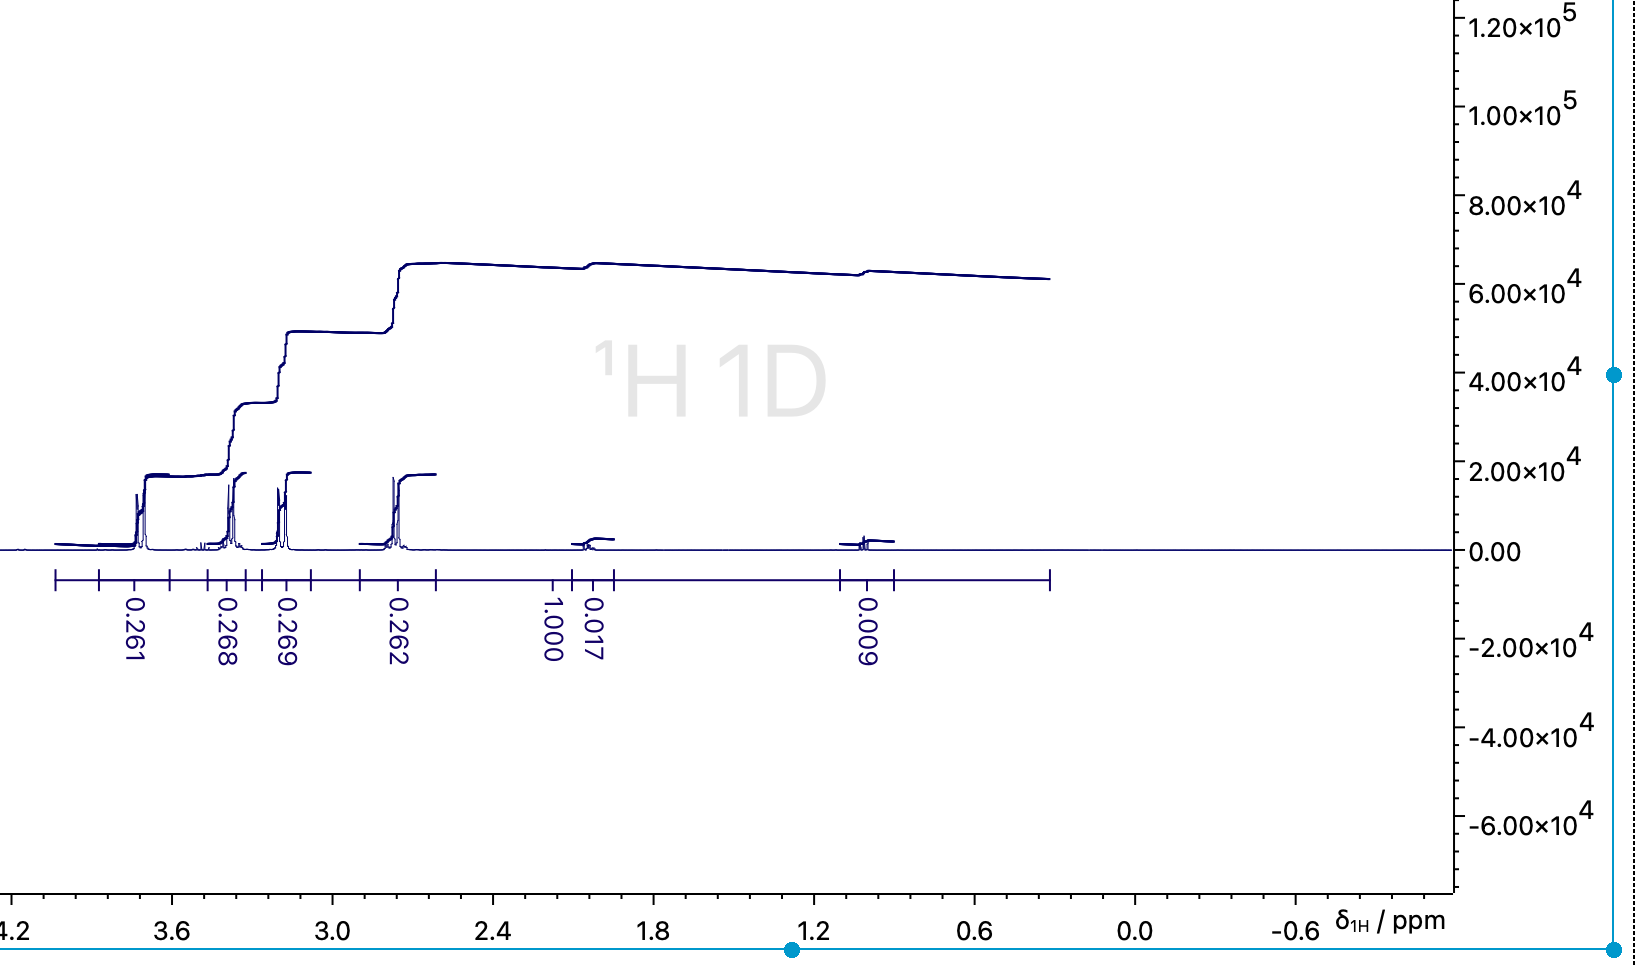
\includegraphics[width=0.8\linewidth]{Relazione/foto/Dinosar_integration_zoom.png}
    \caption{Caption}
    \label{fig:dinosarint}
\end{figure}



\begin{figure}
    \centering
    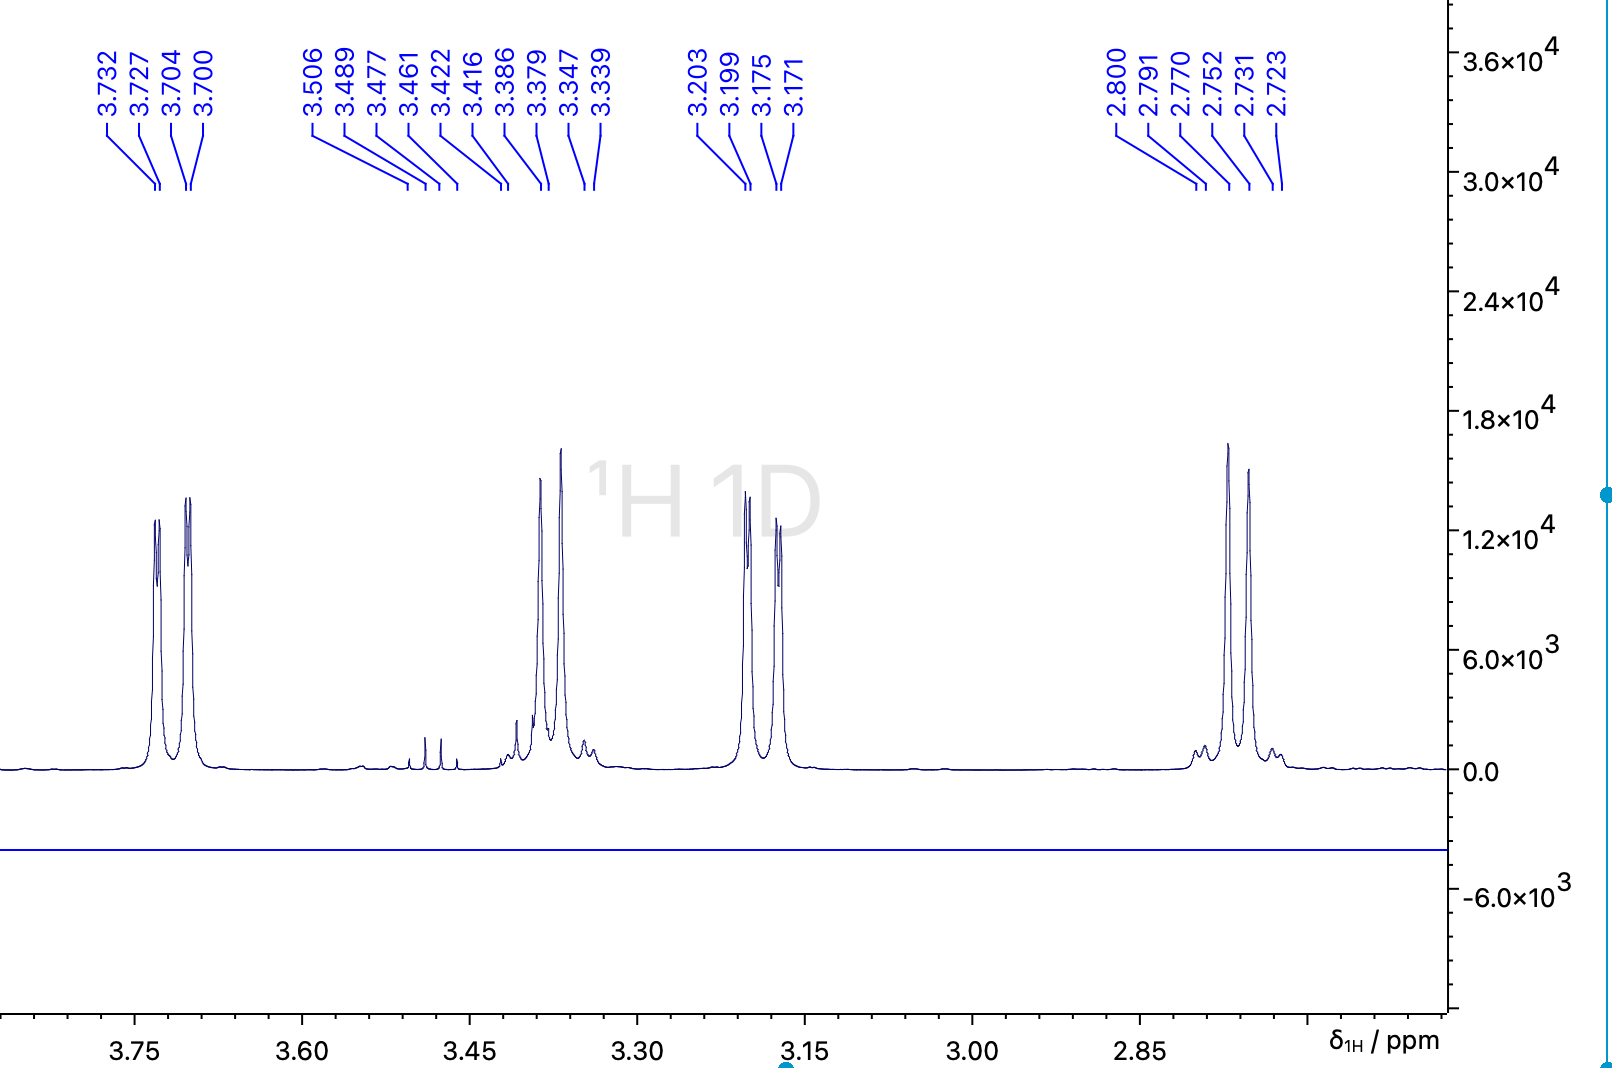
\includegraphics[width=0.8\linewidth]{Relazione/foto/Dinosar_peak_calc.png}
    \caption{Caption}
    \label{fig:dinosarpeakcalc}
\end{figure}

nmr i piccoli picchi posso essere dovuti all'etanolo di lavaggio

